\let\negmedspace\undefined
\let\negthickspace\undefined
\documentclass[journal]{IEEEtran}
\usepackage[a5paper, margin=10mm, onecolumn]{geometry}
%\usepackage{lmodern} % Ensure lmodern is loaded for pdflatex
\usepackage{tfrupee} % Include tfrupee package

\setlength{\headheight}{1cm} % Set the height of the header box
\setlength{\headsep}{0mm}     % Set the distance between the header box and the top of the text
\usepackage{gvv-book}
\usepackage{gvv}
\usepackage{cite}
\usepackage{amsmath,amssymb,amsfonts,amsthm}
\usepackage{algorithmic}
\usepackage{graphicx}
\usepackage{textcomp}
\usepackage{xcolor}
\usepackage{txfonts}
\usepackage{listings}
\usepackage{enumitem}
\usepackage{mathtools}
\usepackage{gensymb}
\usepackage{comment}
\usepackage[breaklinks=true]{hyperref}
\usepackage{tkz-euclide} 
\usepackage{listings}
% \usepackage{gvv}                                        
\def\inputGnumericTable{}                                 
\usepackage[latin1]{inputenc}                                
\usepackage{color}                                            
\usepackage{array}                                            
\usepackage{longtable}                                       
\usepackage{calc}                                             
\usepackage{multirow}                                         
\usepackage{hhline}                                           
\usepackage{ifthen}                                           
\usepackage{lscape}
\begin{document}
	
	\bibliographystyle{IEEEtran}
	\vspace{3cm}
	
	\title{1.1.8.28}
	\author{EE24BTECH11059 - Yellanki Siddhanth
	}
	% \maketitle
	% \newpage
	% \bigskip
	{\let\newpage\relax\maketitle}
	
	\renewcommand{\thefigure}{\theenumi}
	\renewcommand{\thetable}{\theenumi}
	\setlength{\intextsep}{10pt} % Space between text and floats
	
	
	\numberwithin{equation}{enumi}
	\numberwithin{figure}{enumi}
	\renewcommand{\thetable}{\theenumi}
	
	
	\textbf{Question}:\\
	Find the equation of the set of the points $P$ such that its distances from the points
	$A\brak{3, 4, -5}$ and $B\brak{-2, 1, 4}$ are equal.
	\\ \textbf{Solution: }\\
	\begin{table}[h!]    
		\centering
		

		\caption{}
	\end{table}\\
	If \textbf{O} is equidistant from the points \textbf{A} and \textbf{B}
	\begin{align}
		\abs{\abs{\vec{O}-\vec{A}}} = \abs{\abs{\vec{O}-\vec{B}}}\\ \label{eq1.1.8.28.1}
	\end{align}
	\begin{align}
		\abs{\abs{\vec{O}-\vec{A}}}^2 = \abs{\abs{\vec{O}-\vec{B}}}^2\label{eq1.1.8.28.2}\\
	\end{align}
	\begin{align}
		\abs{\abs{\vec{O}}}^2 - 2\vec{O}^\top \vec{A} + \abs{\abs{\vec{A}}}^2 = \abs{\abs{\vec{O}}}^2 - 2\vec{O}^\top\vec{B} + \abs{\abs{\vec{B}}}^2\label{eq1.1.8.28.3}
	\end{align}
	By simplifying further,
	\begin{align}
		\brak{\vec{A}-\vec{B}}^\top O = \frac{\abs{\abs{\vec{A}}}^2-\abs{\abs{\vec{B}}}^2}{2} \label{eq1.1.8.28.4}
	\end{align}
	The above equation is the general expression for the perpendicular bisecting plane between any points $\vec{A}$ and $\vec{B}$.\\
	Substituting the $\vec{A}$ and $\vec{B}$ values in the derived equation.\\
	\begin{align}
		\myvec{5 \\ 3 \\ -9}^\top O = \frac{\abs{\abs{\myvec{3 \\ 4\\-5}}}^2-\abs{\abs{\myvec{-2\\ 1\\4}}}^2}{2} = \frac{29}{2}\label{eq1.1.8.28.5}
	\end{align}
	Comparing with $n^\top x = c$
	\begin{align}
		\vec{n} = \myvec{5 \\ 3 \\ -9}\\ \label{eq1.1.8.28.6}
		\vec{c} = \frac{29}{2}\\    
	\end{align}
	Final Plane equation is:
	
	\begin{align}
		Plane \equiv \myvec{5 \\ 3 \\ -9}^\top\myvec{\vec{x} \\ \vec{y} \\ \vec{z}}= \myvec{14.5}
	\end{align}    
	
	
	\begin{figure}[h]
		\centering
		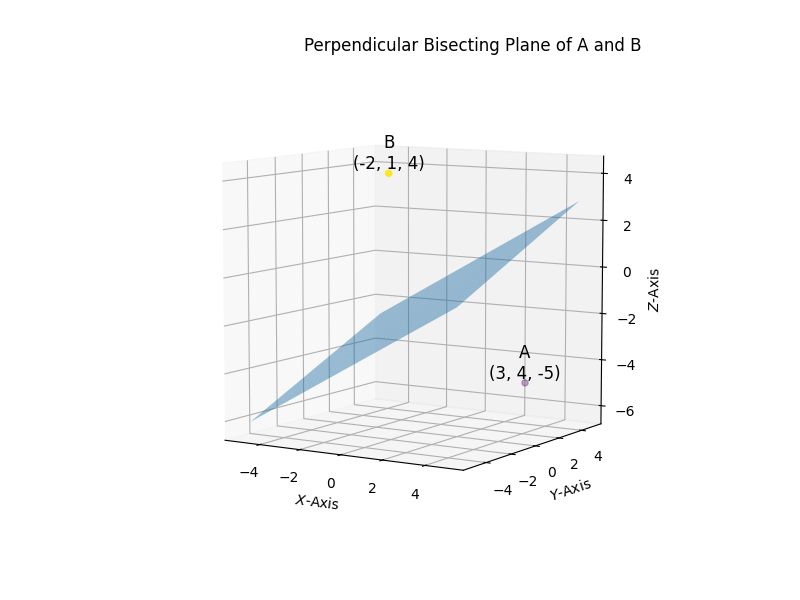
\includegraphics[width=0.7\linewidth]{figs/fig1.png}
		\caption{}
		\label{graph}
	\end{figure}
	
	
	
\end{document}  







